\documentclass[a4paper,11pt]{article}
\usepackage[utf8]{inputenc}
\usepackage[T1]{fontenc}
\usepackage{amsmath}
\usepackage{mathtools}
\usepackage{amsfonts}
\usepackage{amssymb}
\usepackage{graphicx}
\usepackage{multicol}
\usepackage{array}
\usepackage{float}
\usepackage{epstopdf}
\usepackage{caption}
\usepackage{subcaption}
\usepackage{gensymb}
\usepackage[bottom]{footmisc}
\usepackage{appendix}
\usepackage{pdfpages}
\usepackage{todonotes}
\usepackage{mathpazo}
\usepackage{titleps}
\usepackage{color}
\usepackage{xcolor}
\usepackage{colortbl}
\usepackage{siunitx}
\usepackage{pdflscape}
\usepackage{cancel}

\usepackage[skins]{tcolorbox}
\usepackage{sectsty}
\usepackage[arrowmos]{circuitikz}
\usepackage{pgfplots}
\usepackage{blindtext}
\usepackage[inner=2cm,outer=2cm,top=2.5cm,bottom=2.5cm]{geometry}
\usepackage{todonotes}
\usepackage{hyperref}
\usepackage{url}
\usepackage{adjustbox}
\usepackage{tabularx}
\usepackage{booktabs}

\graphicspath{{figs/}}
\sectionfont{\large}
\subsectionfont{\normalsize}



%%%%%%%%%%%%%%%%%%%
% HANDS-ON NUMBER
\newcommand\handsOnN{0}
% WEEK NUMBER
\newcommand\weekN{0}
%%%%%%%%%%%%%%%%%%%

\newpagestyle{main}{
	\sethead[LELEC2102: Hands-on \handsOnN][][Week \weekN]{LELEC2102: Hands-on \handsOnN}{}{Week \weekN}
	\headrule
    \setfoot[][\thepage][]{}{\thepage}{}
}


\newcommand{\horrule}[1]{\rule{\linewidth}{#1}} % Create horizontal rule command with 1 argument of height

\begin{document}
\renewcommand{\figurename}{Fig.}

\renewcommand{\thepage}{\arabic{page}}
\setcounter{page}{1}
\pagestyle{main}
\newpage \clearpage

\begin{center}
\begin{huge}
Hands-On \handsOnN: Installation of Virtual Machine\\
\end{huge}
\vspace{0.3cm}
%\textit{TA 1, TA 2}
\end{center}
\section{Introduction}
In order to simplify the installation of all programs needed for the LELEC2102-3 project, we provide you a Virtual Machine (VM) in which all programs have already been installed. A VM is nothing but an emulation of a full computer system, with its own operating system (Linux in our case). In order to add the VM to your personal computer, you need to install \textit{Oracle VM VirtualBox} and provide it the Disk Image of the VM.\\

\textit{Important remark:} Since a VM contains a full operating system, it is quite heavy. Make sure to have \textbf{at least 20 GB of free disk space}.\\

In order to download \textit{Oracle VM VirtualBox}, use the following link: \href{https://www.virtualbox.org/}{\textcolor{blue}{https://www.virtualbox.org/}}.\\
Click on download Virtual Box 6.1, choose the distribution according to your operating system, download the installer, execute it and follow the different steps.


\section{Configuration of Virtual Machine}
\begin{enumerate}
\item First you need to download the Disk Image of the VM from Moodle. As the file is quite heavy (larger than 15 GB), we suggest you to download it while you are connected to the UCLouvain network (eduroam). Download it in any folder you want (most probably the Download folder).
\item Launch \textit{Oracle VM VirtualBox}.
\item Click on \textit{New}.
\item Enter the following configuration:
\begin{itemize}
\item Give a name to the VM.
\item Choose your VirtualBox folder. You can keep the default one.
\item Select \textit{Linux} as Type.
\item Version is \textit{Ubuntu (64-bit)}.
\item Define the allocated memory for the VM. Please allocate at least 4096MB, you can change this value later if needed.
\item Select \textit{Use an existing virtual hard disk file}. Then add the file by clicking on the icon on the right. A new window opens, click on Add, locate the hard disk image you downloaded previoulsy (in first step) and select Choose.
\end{itemize}

\begin{figure}[H]
    \centering
    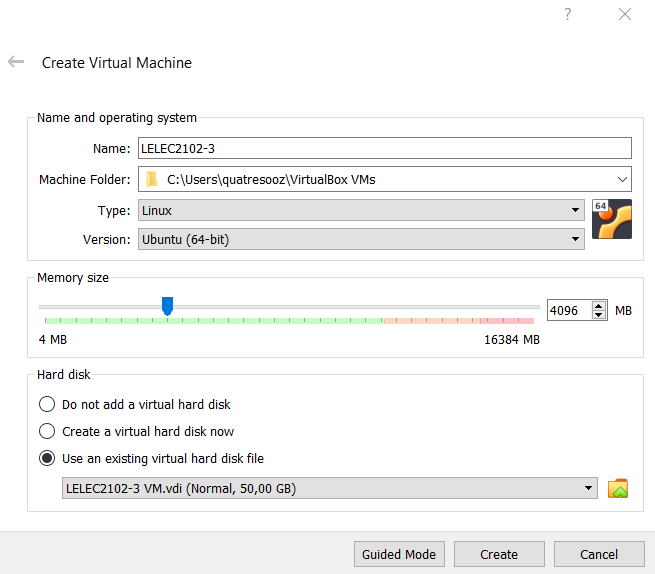
\includegraphics[width=0.8\textwidth]{figs/Capture2.PNG}
	\caption{Creation window of VM.}
	\label{fig1}
\end{figure}

\item Click on Create.
\item In the main window of Virtual Box, you can now select the VM. Then click on Start. If the VM starts properly, follows the next step of this tutorial. In case of an error, close the VM and check the Potential Issues section (just below).

\begin{figure}[H]
    \centering
    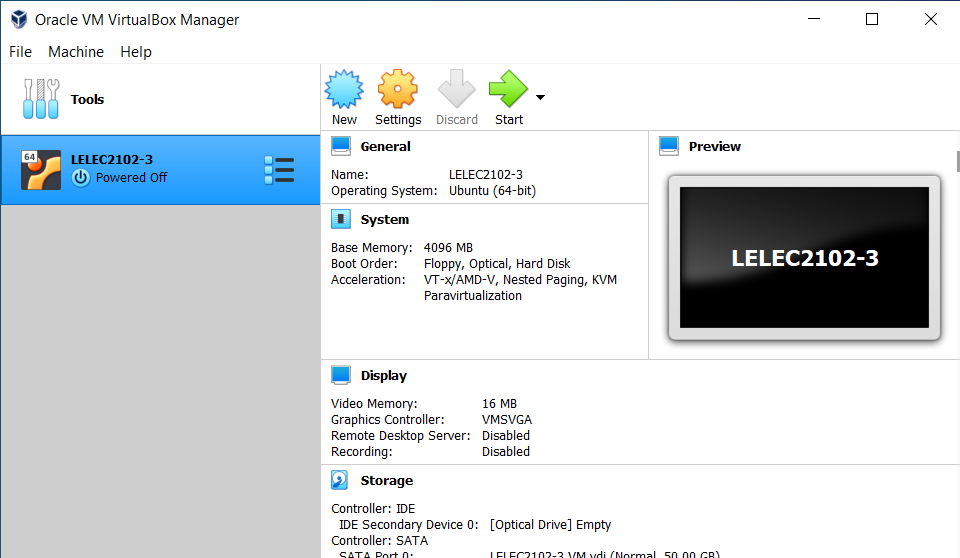
\includegraphics[width=0.8\textwidth]{figs/Capture3.PNG}
	\caption{Main window of VirtualBox.}
	\label{fig2}
\end{figure}

\item The VM opens with lubuntu 20.04. The window size may not be scaled appropriately. You can change it manually by going in the \textit{Monitor settings} (see figure below). Choose the resolution that fits your needs, click on Apply and make sure the changes are OK for you. Click on Save.
\begin{figure}[H]
    \centering
    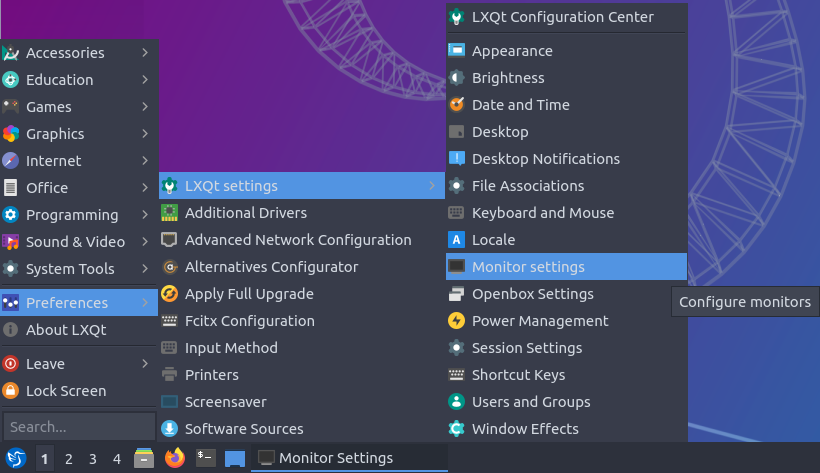
\includegraphics[width=0.8\textwidth]{figs/screen_size.png}
	\caption{How to set screen size in the VM.}
	\label{fig3}
\end{figure}
Locate the bottom right corner of your the VirtualBox window. It should be written which is the \textit{Host key} used by the program, most probably ``CTRL RIGHT''. This key is used for all the shortcuts in the VM. For example, you can make it in Full Screen by pressing ``host key + F''.

\item You are now ready to use all the pre-installed programs that will be useful for the LELEC2102-3 project.
\end{enumerate}
\paragraph{Username and password} The default username is ``marconi''. The password (for admin rights) is ``faraday''.

\section{Potential issues}
If you face some issues during the installation, do not hesitate to ask the teaching assistants. Also, you can add a message on the Moodle forum with full details of the error.

\subsection*{VM is freezing or lagging}
You probably need to allocate more computer resources to the VM. To do so, make sure the VM is closed, go to the Settings tab in the main window of VirtualBox (see Fig. \ref{fig2}). Then, under the System tab, you can increase the memory allocated to the VM (in the Motherboard tab) or increase the number of CPUs (in the Processor tab). Stay in the green area.

\subsection*{Virtualization or Hardware acceleration error message}
In this case, the VM is not starting. Going into the Settings and under the Systems tab, try to enter the Acceleration tab and enable the virtualization. If you can't access the Acceleration tab, you probably need to allow Virtualization or Hardware Acceleration in the BIOS. Please follow the steps given in this \href{https://www.youtube.com/watch?v=XgF7RiXs43k}{\textcolor{blue}{video}}. Equivalently, you can look at the tutorial \href{https://www.bleepingcomputer.com/tutorials/how-to-enable-cpu-virtualization-in-your-computer-bios/}{\textcolor{blue}{here}}.

\textit{Important remark:} Don't do stupid things in the BIOS... The teaching team of the project is not responsible for the changes you may do in the BIOS.

\subsection*{VirtualBox not allowing 64-bits VM}
This could be a virtualization error. Similarly to the issue given above, check that Virtualization is enabled in the BIOS.


\subsection*{Mac-OS: ``Kernel driver not installed''}
You need to allow ``System software from developer Oracle America'' in the Security and Privacy settings. Follow the steps given \href{https://medium.com/@Aenon/mac-virtualbox-kernel-driver-error-df39e7e10cd8}{\textcolor{blue}{here}}.

\section{Some improvements}
If you want to simplify your life while using the VM, you can do the following improvements.
\subsection*{Setting screen size automatically}
It is quite tedious to always change the screen size/resolution to match the one of your computer when launching the VM. You can do it automatically by:
\begin{enumerate}
\item Starting the VM.
\item When the VM has started, go to Devices (top of the VirtualBox window) and click on \textit{Insert Guest Additions CD image...}. A new device will be plugged in the VM. You can access it by opening a terminal, going into the media folder and running VBoxLinuxAdditions.run (with admin rights).
\begin{figure}[H]
    \centering
    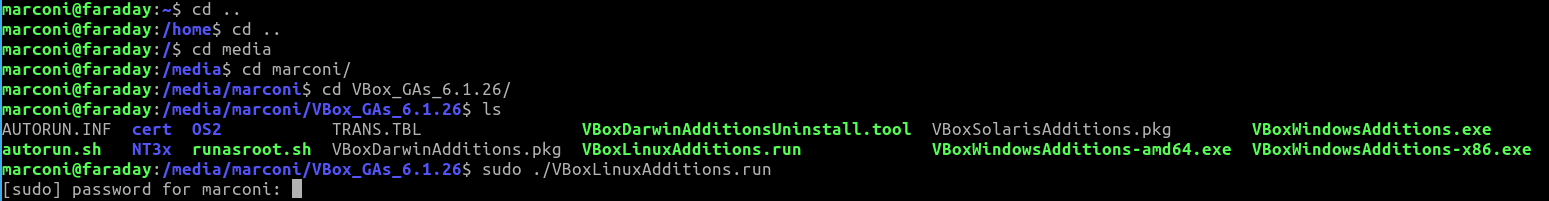
\includegraphics[width=0.95\textwidth]{figs/run_VBOX.PNG}
	\caption{How to run VBoxLinuxAdditions.}
	\label{figrun}
\end{figure}
\item After the run is complete, you need to restart the VM and next time you open it, it should fit your screen perfectly.
\item If you need additional resource, have a look at this \href{https://www.howtogeek.com/howto/2845/install-guest-additions-to-windows-and-linux-vms-in-virtualbox/}{\textcolor{blue}{tutorial}} or this \href{https://www.youtube.com/watch?v=YRK8jtP3B60}{\textcolor{blue}{video}} (but with a Windows VM and not a Linux one).
\end{enumerate}

\subsection*{Copy-Paste and drag-and-drop}
If you want to be able to copy-paste or drag-and-drop from the VM to your computer and the opposite, you first need to install VBoxLinuxAdditions as presented above.
Then, close the VM and in the VirtualBox main window, go to Settings. Under the General tab, go to Advanced and set the Shared Clipboard to \textit{bidirectional}. Do the same for the Drag'n'Drop. You can now start your VM.
If you need more information, have a look \href{https://www.howtogeek.com/187535/how-to-copy-and-paste-between-a-virtualbox-host-machine-and-a-guest-machine/}{\textcolor{blue}{here}}.
\end{document}
